\section{Definitions}
\begin{definitionBox}[Strict sense stationary]
    A random process $\rv{x}(t)$ is called \emph{strict sense stationary} if its statistical properties are invariant to a shift in time. That is,
    \begin{align}
        \pdf{x_{1}, \ldots, x_{n}; t_{1}, \ldots, t_{n}} &=
        \pdf{x_{1}, \ldots, x_{n}; t_{1+\tau}, \ldots, t_{n+\tau}}
    \end{align}
    for any $n$, $t_{1}, \ldots, t_{n}$, and $\tau$.
    % % \index{Strict sense stationary (SSS)}
    % % \index{SSS|see {Strict sense stationary}}
\end{definitionBox}

\begin{definitionBox}[Jointly SSS]
    Two processes $\rv{x}(t)$ and $\rv{y}(t)$ are called \emph{jointly stationary} if the joint statistics of 
    \begin{align}
        \rv{x}(t_{1}), \ldots, \rv{x}(t_{n}), \rv{y}(t_{1}^{\prime}), \ldots, \rv{y}(t_{m}^{\prime})
    \end{align}
    are the same as the joint statistics of 
    \begin{align}
        \rv{x}(t_{1} + \tau), \ldots, \rv{x}(t_{n} + \tau), \rv{y}(t_{1}^{\prime} + \tau), \ldots, \rv{y}(t_{m}^{\prime} + \tau)
    \end{align}
    for any $t_{1}, \ldots, t_{n}$, $n$, $t_{1}', \ldots, t_{m}'$, $m$, and $\tau$. 
    % % \index{Jointly strictly sense stationary}
    % % \index{Strict sense stationary (SSS)!Jointly strictly sense stationary}
\end{definitionBox}

\begin{definitionBox}[Complex stationary]
    A complex process $\rv{z}(t) = \rv{x}(t) + \jmath \rv{y}(t)$ is called \emph{stationary} if the processes $\rv{x}(t)$ and $\rv{y}(t)$ are jointly stationary.
    % % \index{Strict sense stationary (SSS)!Complex stationary}
    % % \index{Complex stationary processes}
\end{definitionBox}

\begin{definitionBox}[Wide sense stationary]
    A random process $\rv{x}(t)$ is called \emph{wide sense stationary (WSS)} if 
    \begin{enumerate}
        \item its mean is constant
        \begin{align}
            \expect{\rv{x}(t)} &= \eta,
        \end{align}
        and
        \item its autocorrelation function $\acor{t_{1}}[t_{2}]$ depends only on $t_{1} - t_{2}$. That is,
        \begin{align}
            \expect{\rv{x}(t_{1})\rv{x}(t_{2})^{\herm}} &= \acor{t_{1}-t_{2}},
        \end{align}
        or equivalently
        \begin{align}
            \expect{\rv{x}(t+\tau)\rv{x}^{\herm}} &= \acor{\tau}.
        \end{align}
    \end{enumerate}
    % % \index{Wide sense stationary (WSS)}
\end{definitionBox}

\begin{remarkBox}
    A SSS process is also WSS. However, the inverse is true only for Gaussian process.
\end{remarkBox}

\begin{definitionBox}[Crosscorrelation]
    Let $\rv{x}(t)$ and $\rv{y}(t)$ be two random processes. The \emph{cross-correlation} $\acor[xy]{t_{1}}[t_{2}]$ of $\rv{x}(t)$ and $\rv{y}(t)$ is
    \begin{align}
        \acor[xy]{t_{1}}[t_{2}] &= \expect{\rv{x}(t_{1})\rv{y}(t_{2})^{\herm}}.
    \end{align}
\end{definitionBox}

\begin{definitionBox}[Joinly WSS]
    Two processes $\rv{x}(t)$ and $\rv{y}(t)$ are called jointly WSS if
    \begin{enumerate}
        \item each one of them is WSS, and
        \item their cross-correlation function $\acor[xy]{t_{1}}[t_{2}]$ depends only on $t_{1}-t_{2}$. That is,
        \begin{align}
            \expect{\rv{x}(t_{1})\rv{y}(t_{2})^{\herm}} &= \acor[xy]{t_{1}-t_{2}},
        \end{align}
        or, equivalently,
        \begin{align}
            \acor[xy]{t+\tau}[t] &= \expect{\rv{x}(t+\tau)\rv{y}(t)^{\herm}}\\
            &= \acor[xy]{\tau}.
        \end{align}
    \end{enumerate}
\end{definitionBox}
\begin{remarkBox}
    Some properties of WSS processes. 
    
    \begin{itemize}
        \item For $\tau=0$,
        \begin{align}
            \expect{\abs{\rv{x}(t)}^{2}} &= \acor{0}.
        \end{align}
        \item $\acor{\tau} = \acor{-\tau}^{\herm}$.
        \item For a real WSS random processes, the autocorrelation function is an even function of $\tau$. 
        \item The autocorrelation function of a real random process is maximized at $\tau=0$. That is,
        \begin{align}
            \acor{0} \geq \acor{\tau}.
        \end{align}
        Furthermore,
        \begin{align}
            \acor{0}\geq \abs{\acor{\tau}}.
        \end{align}
    \end{itemize}
\end{remarkBox}
\begin{definitionBox}[Power spectral density (PSD)]
    The \emph{power spectrum} or \emph{power spectral density} (PSD) of a WSS process $\rv{x}(t)$ (real or complex) is the Fourier transform $\psd[xx]{\omega}$ of its autocorrelation $\acor[xx]{\tau} = \expect{\rv{x}(t+\tau)\rv{x}(t)^{\herm}}$. That is,
    \begin{align}
        \psd[xx]{\omega} &= \fouriert{\acor[xx]{\tau} }\\
        &= \int_{-\infty}^{\infty}\acor[xx]{\tau}e^{-\jmath\omega\tau}\dee\tau.
    \end{align}
    The autocorrelation function can be obtained from the PSD using the inverse Fourier transform. Specifically,
    \begin{align}
        \acor[xx]{\tau} &= \invfouriert{\psd[xx]{\omega}}\\
        &= \f{1}{2\pi} \int_{-\infty}^{\infty} \psd[xx]{\omega}e^{\jmath\omega\tau}\dee\omega.
    \end{align}
\end{definitionBox}

\begin{remarkBox}
    Some properties of the power spectral density.
    \begin{itemize}
        \item Since $\acor[xx]{\tau}^{\herm} = \acor[xx]{-\tau}$, then 
        \begin{align}
            \psd[xx]{\omega}^{\herm} &= \psd[xx]{\omega}.
        \end{align}
        That is, the PSD is always a real function of $\omega$.
    \end{itemize}
    \item If $\rv{x}(t)$ is a real process, then the PSD is a \emph{real} and \emph{even} function of $\omega$.
\end{remarkBox}


\begin{definitionBox}[Cross PSD]
    The \emph{cross power spectrum} or \emph{cross power spectral density} of the jointly WSS processes $\rv{x}(t)$ and $\rv{y}(t)$ is the Fourier transform, $\psd[xy]{\omega}$ of their cross-correlation. That is,
    \begin{align}
        \psd[xy]{\omega} &= \fouriert{\acor[xy]{\tau}}\\
        &= \int_{-\infty}^{\infty} \acor[xy]{\tau}e^{-\jmath\omega\tau}\dee\tau.
    \end{align}
    The cross-correlation function can be computed from the cross PSD using the inverse Fourier transform. That is,
    \begin{align}
        \acor[xy]{\tau} &= \invfouriert{\psd[xy]{\omega}}\\
        &= \f{1}{2\pi}\int_{-\infty}^{\infty}\psd[xy]{\omega}e^{\jmath\omega\tau}\dee\omega.
    \end{align}
    In general, the cross PSD is a complex function of $\omega$ with the property
    \begin{align}
        \psd[xy]{\omega} &= \psd[yx]{\omega}^{\herm}.
    \end{align}
\end{definitionBox}


\section{Theorems}
\begin{theoremBox}
   [Wiener-Kinchin]    
     For any random process $\rv{x}(t)$, 
     \begin{align}
         \psd[xx]{\omega}\geq 0.
     \end{align}
\end{theoremBox}

\begin{theoremBox}
   [Existence of PSD]    
     Given any arbitrary finite\footnote{I.e., $\int\psd{\omega}\dee\omega<\infty$.} positive function $\psd{\omega}$, there exists a complex process $\rv{x}(t)$ with PSD $\psd[xx]{\omega}$ equal to $\psd{\omega}$.
\end{theoremBox}


\section{Deterministic systems}
\begin{figure}[H]
    \centering
    \begin{subfigure}{0.35\textwidth}
        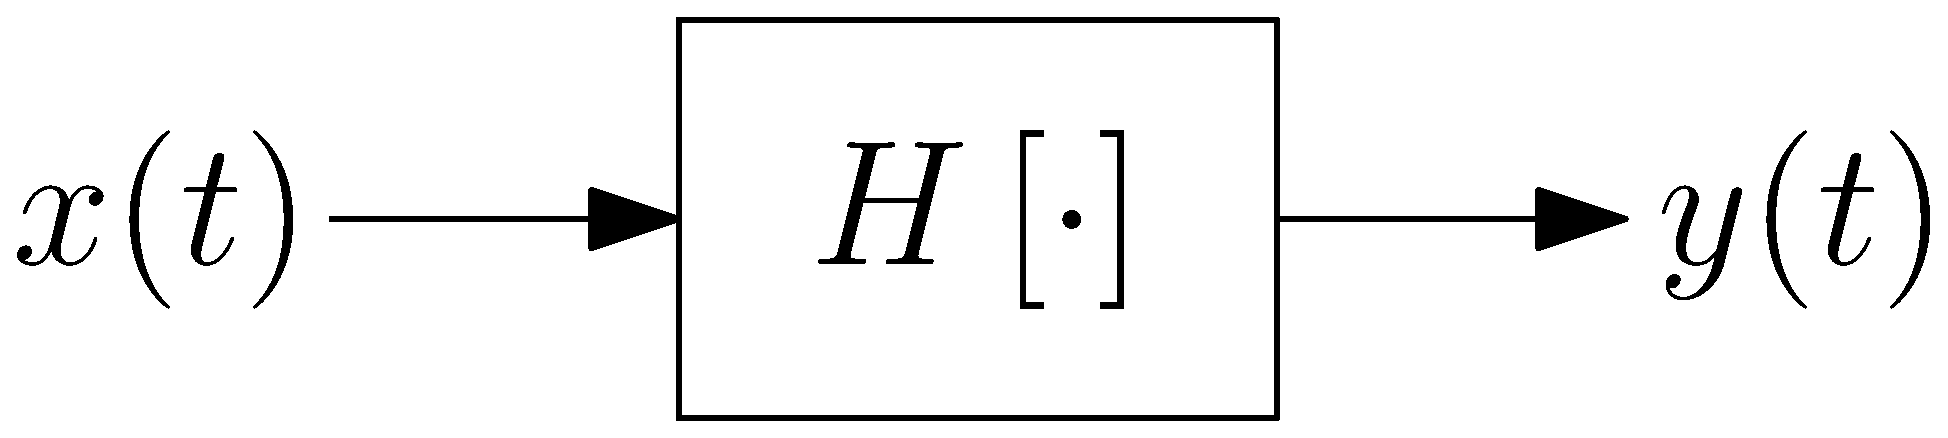
\includegraphics[width=\textwidth]{figs/determenistic_system_det_input.eps}
        \caption{Deterministic input}
        \label{fig:determenistic_system_det_input}
    \end{subfigure}
    \hspace{1cm}
    \begin{subfigure}{0.35\textwidth}
        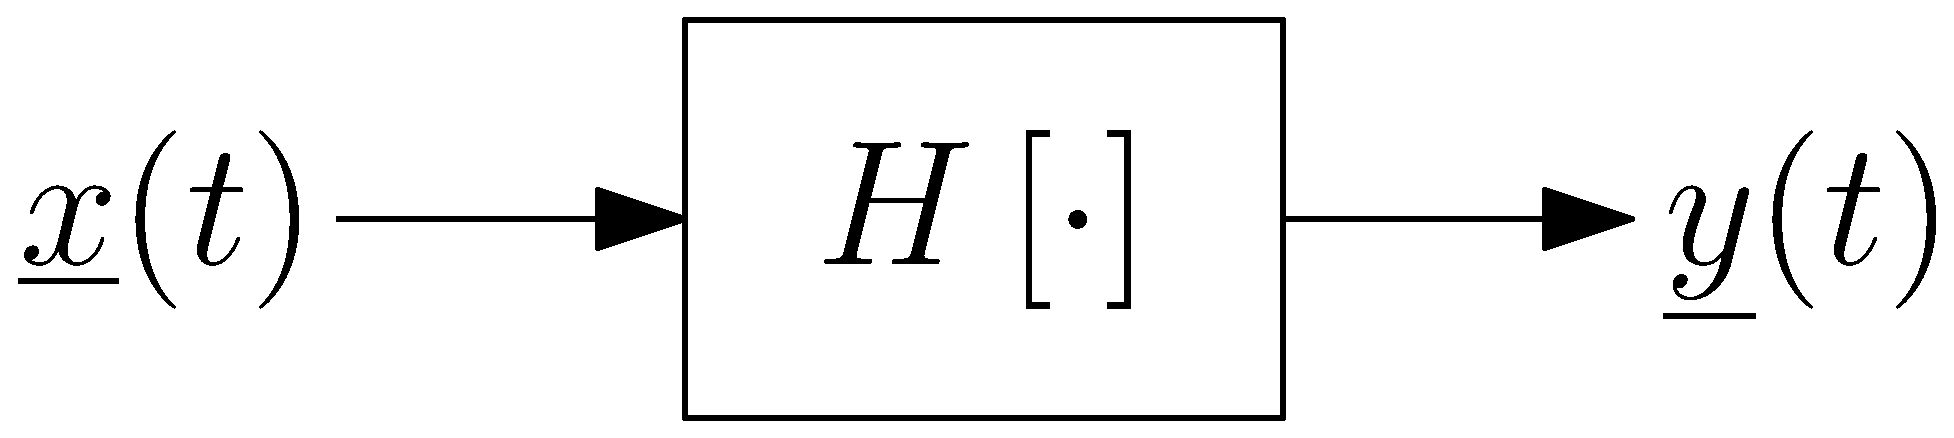
\includegraphics[width=\textwidth]{figs/determenistic_system_rand_input.eps}
        \caption{Random input}
        \label{fig:determenistic_system_rand_input}
    \end{subfigure}
    \caption{Deterministic system schematic.}
    \label{fig:deterministic system schematic}
\end{figure}
\begin{definitionBox}[System]
    A system is an object, or a set of functions, that take an input function $x(t)$ and outputs an output function $y(t)$. 
    
    The function can be deterministic as seen in Figure~\ref{fig:determenistic_system_det_input}, or stochastic as seen in Figure~\ref{fig:determenistic_system_rand_input}.
\end{definitionBox}
% \index{System}

\begin{remarkBox}
    The notation 
    \begin{align}
        \rv{y}(t) &= H\left[ \rv{x}(t) \right]]
    \end{align}
    reads ``system $H$ applied on input $\rv{x}(t)$ to give the output $\rv{y}(t)$.''
\end{remarkBox}
\begin{definitionBox}[Deterministic systems]
    A system is called \emph{deterministic} if, identical realizations of the input process $\rv{x}(t)$ yield identical realizations of the output process $\rv{y}(t)$.
\end{definitionBox}
% \index{System}
% \index{Deterministic system}

\begin{definitionBox}[Stochastic system]
    A system that is not deterministic is called \emph{stochastic}.
\end{definitionBox}
% \index{Stochastic system}

\begin{definitionBox}[Linear system]
    A system $L$ is called \emph{linear} if it satisfies the scaling and superposition property. That is, for any random scalers $\rv{a}_{1}$, $\rv{a}_{2}$ and random processes $\rv{x}_{1}(t)$, $\rv{x}_{2}(t)$, the following holds
    \begin{align}
        L\left[ \rv{a}_{1}\rv{x}_{1}(t) + \rv{a}_{2}\rv{x}_{2} \right]
        &= 
        \rv{a}_{1}L\left[ \rv{x}_{1}(t) \right] + \rv{a_{2}}L\left[ \rv{x}_{2}(t) \right].
    \end{align}
\end{definitionBox}
% \index{Linear system}

\begin{theoremBox}
   [Fundamental theorem]    
     For any linear system $L$ the following property holds.
     \begin{align}
         \expect{L\left[ \rv{x}(t) \right]} &= L\left[ \expect{ \rv{x}(t)} \right].
     \end{align}
\end{theoremBox}

\subsection{Input-output cross-correlation}
The input-output cross-correlation is given by
\begin{align}
    \acor[xy]{t_{1}}[t_{2}] &= \expect{\rv{x}(t_{1})\rv{y}(t_{2})}.
\end{align}
The output at $t_{2}$ is denoted by
\begin{align}
    \rv{y}(t_{2}) &= \left.L\left[ \rv{x}(t) \right]\right|_{t=t_{2}}\\
    &= L_{t_{2}}\left[ \rv{x}(t_{2}) \right].
\end{align}
The subscript $t_{2}$ on $L$ denotes that the linear system operates on functions of $t_{2}$. Any other functions are treated as scalars.
Thus, 
\begin{align}
    \rv{x}(t_{2})\rv{y}(t_{2}) &= \rv{x}(t_{1})L_{t_{2}}\left[ \rv{x}(t_{2}) \right]\\
    &= L_{t_{2}}\left[ \rv{x}(t_{1})\rv{x}(t_{2}) \right],
\end{align}
where $\rv{x}(t_{1})$ was treated as a scaler in $L_{t_{2}}$.

Therefore,
\begin{blueBox}
    \begin{align}
        \acor[xy]{t_{1}}[t_{2}] &= \expect{\rv{x}(t_{1})\rv{y}(t_{2})} \\
        &= \expect{ L_{t_{2}}\left[ \rv{x}(t_{1})\rv{x}(t_{2}) \right]}\\
        &= L_{t_{2}}\left[ \expect{\rv{x}(t_{1})\rv{x}(t_{2})} \right]\\
        &= L_{t_{2}}\left[ \acor[xx]{t_{1}}[t_{2}] \right].
    \end{align}
\end{blueBox}

\subsection{Output autocorrelation}
THe output autocorrelation 
\begin{align}
    \acor[yy]{t_{1}}[t_{2}] &= \expect{\rv{y}(t_{1})\rv{y}(t_{2})}
\end{align}
is given as follows.

The output at $t_{1}$ is given by
\begin{align}
    \rv{y}(t_{1}) &= L_{t_{1}}\left[ \rv{x}(t_{1}) \right].
\end{align}
Therefore, 
\begin{align}
    \rv{y}(t_{1})\rv{y}(t_{2}) &= L_{t_{1}}\left[ \rv{x}(t_{1}) \right]\rv{y}(t_{2})\\
    &= L_{t_{1}}\left[ \rv{x}(t_{1})\rv{y}(t_{2}) \right].
\end{align}
Therefore,
\begin{align}
    \expect{ \rv{y}(t_{1}) \rv{y}(t_{2})} 
    &= \expect{ L_{t_{1}}\left[ \rv{x}(t_{1}) \rv{y}(t_{2}) \right]} \\
    &= L_{t_{1}}\left[ \expect{ \rv{x}(t_{1})\rv{y}(t_{2})} \right]\\
    &= L_{t_{1}}\left[ \acor[xy]{t_{1}}[t_{2}] \right]\\
    &= L_{t_{1}}\left[ L_{t_{2}}\left[ \acor[xx]{t_{1}}[t_{2}] \right] \right].
\end{align}
\begin{blueBox}
    That is,
    \begin{align}
        \acor[yy]{t_{1}}[t_{2}] &= L_{t_{1}}\left[ L_{t_{2}}\left[ \acor[xx]{t_{1}}[t_{2}] \right] \right].
    \end{align}
\end{blueBox}

\begin{example}
    Consider the linear system 
    \begin{align}
        \rv{y}(t) &= L\left[ \rv{x}(t) \right]\\
        &= \rv{x}(t) - \rv{x}(t-1).
    \end{align}
    Find
    \begin{enumerate}
        \item the mean of $\rv{y}(t)$, 
        \item the input-output cross-correlation, and
        \item the output autocorrelation.
    \end{enumerate}

    \textbf{Solution}
    The mean of $\rv{y}(t)$ is given by
    \begin{align}
        \expect{\rv{y}(t)} &= \expect{L\left[ \rv{x}(t) \right]}\\
        &= L\left[ \expect{ \rv{x}(t)} \right]\\
        &= \expect{\rv{x}(t)} - \expect{\rv{x}(t-1)}.
    \end{align}
    The input-output cross-correlation is given by
    \begin{align}
        \acor[xy]{t_{1}}[t_{2}] &= L_{t_{2}}\left[ \acor[xx]{t_{1}}[t_{2}] \right] - \acor[xx]{t_{1}}[t_{2}].
    \end{align}
    Note that inside the system $L_{t_{2}}$, the function $\acor[xx]{t_{1}}[t_{2}]$ is treated as a function of a single variable ($t_{2}$). That is, it's as if a function $g(t_{2}) \coloneq \acor[xx]{t_{1}}[t_{2}]$ is defined and passed through the system $L_{t_{2}}\left[ g(t_{2}) \right]$.

    Alternatively,
    \begin{align}
        \acor[xy]{t_{1}}[t_{2}] &= \expect{\rv{x}(t_{1})\rv{y}(t_{2})}\\
        &= \expect{\rv{x}(t_{1})\left[ \rv{x}(t_{2}) - \rv{x}(t_{2}-1) \right]}\\
        &= \expect{ \rv{x}(t_{1})\rv{x}(t_{2}) - \rv{x}(t_{1})\rv{x}(t_{2}-1)}\\
        &= \acor[xx]{t_{1}}[t_{2}] - \acor[xx]{t_{1}}[t_{2}-1].
    \end{align}

    The output autocorrelation is given by
    \begin{align}
        \acor[yy]{t_{1}}[t_{2}] &= L_{t_{1}}\left[ \acor[xy]{t_{1}}[t_{2}] \right]\\
        &= \acor[xy]{t_{1}}[t_{2}] - \acor[xy]{t_{1}-1}[t_{2}]\\
        &= \acor[xx]{t_{1}}[t_{2}] - \acor[xx]{t_{1}-1}[t_{2}]  \nonumber\\&\qquad
        - \acor[xx]{t_{1}}[t_{2}-1] + \acor[xx]{t_{1} - 1}[t_{2} - 1].
    \end{align}
\end{example}

\begin{example}[Differentiator]
    Consider the differentiator system $L$
    \begin{align}
        \rv{y}(t) &= L\left[ \rv{x}(t) \right]\\
        &= \td{}{t}\rv{x}(t).
    \end{align}
    Find
    \begin{enumerate}
        \item the mean of $\rv{y}(t)$, and
        \item the input-output cross-correlation.
    \end{enumerate}
    \textbf{Assumption}: all realizations of $\rv{x}(t)$ are differentiable.

    \textbf{Solution}. The mean of the derivative of $\rv{x}(t)$ is given by
    \begin{align}
        \expect{\rv{y}(t)} &= \expect{L\left[ \rv{x}(t) \right]}\\
        &= L\left[ \expect{ \rv{x}(t)} \right]\\
        &= \td{}{t}\expect{\rv{x}(t)}.
    \end{align}
    The input-output cross-correlation is given by
    \begin{align}
        \acor[xy]{t_{1}}[t_{2}] &= L_{t_{2}}\left[ \acor[xx]{t_{1}}[t_{2}] \right]\\
        &= \pd{}{t_{2}}\acor[xx]{t_{1}}[t_{2}].
    \end{align}
\end{example}


\subsection{Linear time-invariant systems}
Linear time-invariant (LTI) systems are 
\begin{itemize}
    \item characterized by impulse response $h(t)$.
    \item The output can be expressed as a convolution with the impulse response. That is,
    \begin{align}
        \rv{y}(t) &= \rv{x}(t) \ast h(t)\\
        &= \int_{-\infty}^{\infty}\rv{x}(t - \alpha)h(\alpha)\dee\alpha.
    \end{align}
    \item The input-output cross-correlation is given by
    \begin{align}
        \acor[xy]{t_{1}}[t_{2}] &= L_{t_{2}}\left[ \acor[xx]{t_{1}, t_{2}} \right]\\
        &= \acor[xx]{t_{1}, t_{2}}\ast h(t_{2})\\
        &= \int_{-\infty}^{\infty} \acor[xx]{t_{1}}[t_{2} - \beta]h(\beta)\dee\beta.
    \end{align}
    \item The output autocorrelation is given by
    \begin{align}
        \acor[yy]{t_{1}}[t_{2}] &= L_{t_{1}}\left[ \acor[xy]{t_{1}}[t_{2}] \right]\\
        &= \acor[xy]{t_{1},t_{2}}\ast h(t_{1})\\
        &= \int_{-\infty}^{\infty} \acor[xy]{t_{1} - \alpha, t_{2}} h(\alpha)\dee\alpha\\
        &= \int_{\infty}^{\infty}\int_{-\infty}^{\infty} \acor[xx]{t_{1} - \alpha}[t_{2} - \beta]h(\alpha)h(\beta)\dee\alpha\dee\beta.
    \end{align}
\end{itemize}

\begin{theoremBox}
     Consider a LTI system with impulse response $h(\tau)$ such tat $\int_{\infty}^{\infty}h(\tau)\dee\tau<\infty$. If the input process $\rv{x}(t)$ is WSS then $\rv{x}(t)$ and the output process $\rv{y}(t)$ are jointly WSS with 
     \begin{align}
         \acor[xy]{\tau} &= \acor[xx]{\tau}\ast h(-\tau),
     \end{align}
     and
     \begin{align}
         \acor[yy]{\tau} &= \acor[xy]{\tau}\ast h(\tau)\\
         &= \acor[xx]{\tau}\ast h(\tau) \ast h(-\tau).
     \end{align}
\end{theoremBox}

\subsection{Power spectra}
Consider a LTI system with the impulse response $h(t)$ such the input $\rv{x}(t)$ is WSS process and the output is $\rv{y}(t)$. Then,
\begin{align}
    \acor[xy]{\tau} &= \acor[xx]{\tau}\ast h(-\tau)^{\herm}\\
    \acor[yy]{\tau} &= \acor[xy]{\tau}\ast h(\tau).
\end{align}
Let $H(\omega)$ be the transfer function\footnote{The Fourier transform of $h(t)$.} of the impulse response. Then,
\begin{align}
    \psd[xy]{\omega} &= \psd[xx]{\omega}H^{\herm}(\omega),\\
    \psd[yy]{\omega} &= \psd[xy]{\omega}H(\omega)\\
    &= \psd[xx]{\omega}\abs{ H(\omega)}^{2}.
\end{align}
Note that since both $\psd[xx]{\omega}$ and $\psd[yy]{\omega}$ are positive and real, then it makes sense that $\abs{ H(\omega)}^{2}$, the term multiplying $\psd[xx]{\omega}$, is positive and real as well.